\documentclass[11pt]{article}
\usepackage[utf8]{inputenc}
\usepackage[T1]{fontenc}
\usepackage[francais]{babel}
\usepackage[francais]{layout}
\usepackage{hyperref}
\selectlanguage{french}

% NE PAS CHANGER !!
% \ifx \public \undefined \def\public{enseignants} \fi
\ifx \public \undefined \def\public{} \fi
\usepackage[\public]{tps}

% Numéro du TP
\newcommand{\numtd}{01 (part one of two)}
% Titre du TP
\newcommand{\titretd}{The command line in Linux}



\begin{document}

\entete{\numtd}{\titretd}

\begin{introduction}
This is the first of a two-part introduction to the GNU/Linux operating system installed on the machines of the Computer Science department. 
It gives you some basic knowledge that you will use throughout your courses. All notions discussed here will be considered as acquired and mastered for all future courses regardless of the module.

\noindent This first TP invites you to (re)discover the command line (shell).

%The computer workstations in Room 411 operate under Xubuntu Xenial 16.04. It is a GNU/Linux operating system (Linux kernel and GNU tools) based on the Ubuntu distribution (a "Debian like") using the Xfce Desktop Environment.

\noindent Connecting to your session gives you access to your work environment. You will need to open a shell (Terminal) to enter the instructions of this TP.	
	

\end{introduction}


\section{First steps}
\subsection{File System}
In Linux everything is a file, where directories are files that contain names of other files. In order to manage these files in an orderly fashion, we like to imagine them as an ordered tree. Each vertex is a file and folders(which are also files) are vertices that can have other children.
The root of the file system is the "root" folder, denoted by "/". Under it you will find all the rest of the files. Let's go over few of the important(for this TP) sub-directories of the root:

\begin{itemize}
	\item {\bf /home}: Where you will find your users’ personal directories.
	\item {\bf /home/"username"}: Your private folder. In most shells(explained soon) the character "\textasciitilde" is interpreted as the path to your privet directory. 
	\item {\bf /bin:} Here you will find most of the commands(applications) that we'll use during this TP.
	
\end{itemize}

\begin{center}
	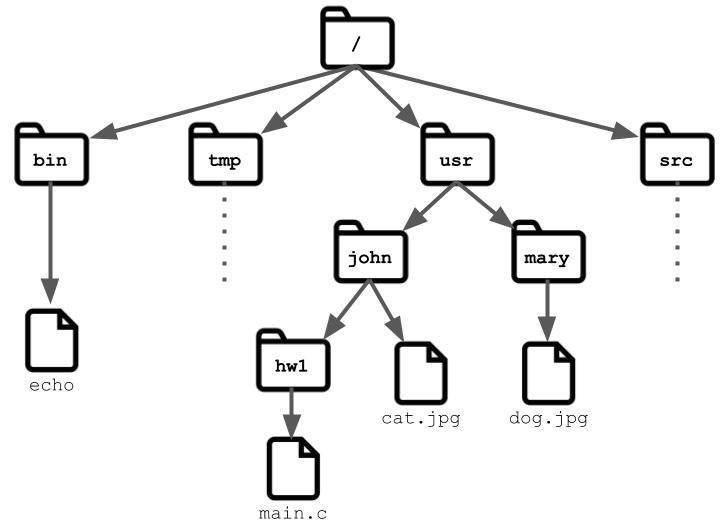
\includegraphics[scale=0.3]{file_tree.png}
\end{center}
\subsection{Shell and Terminal}
 A Terminal is a type of "text input/output environment", which means it can read your textual input and output some text on the screen. In it we'll input our commands to the computer, and get results.
 To open the terminal on you computer(one of the ways), you press "Ctrl+Alt+T". 
 
\noindent The terminal doesn't perform your commands, but sends them to a Shell. The shell is a "command line interpreter", meaning it receives your textual commands and tries to interpret and preform your commands. You can think of it as the steering wheel of you computer. There are multiple types of shells(Sh,Zsh,Ksh\ldots), we are going to use Bash. 
 
 A few tricks that can be useful while using the shell:
 \smallskip
 \begin{itemize}
 	\item {\bf Tab}: While writing you command you can click the Tab button, and the shell will try to auto-complete your command. If it has a multiple options for completion it will do nothing. But, clicking it twice will print out all of the options it found.
 	\item {\bf Ctrl+C \& Ctrl+V}: You'll find out that these two shortcuts don't work 'normally'. This is partially since "Ctrl+C" is designated for stop running process. Instead you can use "Ctrl+Shift+C" and "Ctrl+Shift+V".
 	\item {\bf Special folder shortcuts:} As described earlier, "\textasciitilde" is understood as the address of your home directory. Other shortcuts are "." (current folder), ".." (previous folder).
 	
 \end{itemize}
 

\section{Command line: first steps}
Since the shell is a command line interpreter, to make the shell do something you’ll need to write a
command and send it to the interpreter by pressing "Enter". For example enter the command "ls", what do
you think it does ? 

Some commands have "flags" or "option argument strings" usually beginning with “-”. The flags modify
the behavior of the program being invoked. For example enter the command "ls" with the flag "-l", what
changed ?



\subsection{Finding help}

One of the ways of getting help with the commands on Linux, is to RTFM(read the fine manual). The
manual can be accessed from the shell via the \textbf{man} command(short for manual).


\subsubsection{Man pages}
%Translation
Run the command: \textbf{man man}. What do you see? \\ To search for text, press the key "/" followed by your search query, use the keys \textbf{n} and \textbf{p} to navigate between
different occurrences. \\ To quit the man page press "q."

\begin{solution}
These pages provide the man manual. This command provides help with using commands.
\end{solution}

\subsubsection{Using the man pagesl}
All pages in \textbf{man} are organized in the same way.


\begin{enumerate}
	\item{NAME}: name of the command;
	\item{SYNOPSIS}: short summary of the syntax of the command;
	\item{DESCRIPTION}: long or short description of the command;
	\item{OPTIONS}(optional): description of supported options;
	\item There is of course the possibility to put as many subsections as you want;
	\item{AUTHOR}: the people who developed the command;
	\item{SEE ALSO}: Cross references.	

\end{enumerate}

\subsubsection{Manual of the command \textbf{ls}}

Read the help page for the command "ls" and try to find information that answers the following questions:

\begin{enumerate}
	\item In no more than 10 words, what is the purpose of this command?
	\item Which will print all the files (even those hidden: those whose name starts with a point)?
	\item Which option will print the files with a long listing format ?
	\item Which option will print the size of the files in a human readable way?
	\item Which option will print the subdirectories of the given directory recursively?

\end{enumerate}

\begin{solution}
 \begin{enumerate}
  \item List the contents of a directory
  \item all : ls -a
  \item long listing format : ls -l
  \item human readable : ls -h
  \item recursive : ls -R
 \end{enumerate}
\end{solution}


\subsubsection{Other ways to get help}
There are other option to find help:
\begin{enumerate}
	\item Adding the options - -help in the end of a command gives you a short explanation about this command(mkdir --help).
	\item The command "whatis" displays a one-line description of the command following it (whatis ls).
	\item Using your favorite search engine on the internet, e.g. www.duckduckgo.com, www.bing.com(really ?),
www.google.com,. . .
	\item Asking a fellow human.
\end{enumerate}


\subsubsection{The command \textbf{cd}}

\begin{itemize}
\item Find out what this command is for.
\item Go to the \textbf{tmp} directory at the root of the system and list its contents
\item Return to your home directory
\item What does \textbf{cd -} do?
\end{itemize}


\subsubsection{Wildcards}
A {\bf wildcard} is a symbol that takes the place of an unknown character or set of characters. Some of the heavily used wildcards are:
\begin{itemize}
	\item The asterisk "*", represents any number of unknown characters. For example "*cake" can stand for "carrotcake, chocolatcake,cake,..." and "cake*" can stand for "cakeParty, cakeWorld,cake,...".
	\item The question mark "?", represents only one character. For example "??ke" can stand for "cake,bake,take,\ldots" and "ke??" can stand for "keen,kept,keep,\ldots". 
\end{itemize}
\smallskip

Use the "wildcard" "*" to list all the files starting with "u" in the root of your system.

\begin{solution}
	ls -d /u*
\end{solution}


\begin{solution}
 \begin{itemize}
\item A change of current directory
\item cd /tmp; ls
\item cd or cd \textasciitilde{} or cd /users/dptinfo/$<$login$>$
\item returns to /tmp and more generally returns to the previous directory.
 \end{itemize}
\end{solution}

\subsubsection{Manuel of the command \textbf{mkdir}}

Consider that we want to create at the root of your account the following path:

\begin{lstlisting}
ArchiSys/tp/01
\end{lstlisting}

\noindent Launch the following command and observe what is happening:
                                                         
\begin{lstlisting}
cd ; mkdir ArchiSys/tp/01
\end{lstlisting}
\begin{solution}
Failed to create directory because parent directories do not exist
\end{solution}
\noindent Look in the "mkdir" man page for the option to create the entire directory hierarchy in one command.

\begin{solution}
mkdir -p ArchiSys/tp/01
\end{solution}

\subsection{The command echo}
\noindent
What is the command "echo" used for?

\begin{solution}
Displays a string of characters on the screen possibly substituting variables and interpreting sequences.
\end{solution}

\noindent What does the following command do? Why ?

\begin{lstlisting}[alsoletter={*},emph={*}]
echo -ne "\n\n *\tHello World $LOGNAME\t\t*\n\n"
\end{lstlisting}

\noindent Try the following commands, what is the difference? Why ?

\begin{lstlisting}[alsoletter={*},emph={*}]
echo -e '\n\n *\tHello World $LOGNAME\t\t*\n\n'
\end{lstlisting}

\begin{solution}
	Displays * Hello World <login> * "preceded by 2 blank lines and followed by a single car -n deletes the echo-linked carriage return when we made a carriage return to validate our order.
	
	Second command does not replace the login variable because we are dealing with single quotes. The text is centered because we removed the -n.
	
	We will come back later to the usage of variables in the shell.

\end{solution}

\subsection{Other commands}

In the following, we will use the command "ps" which lists the programs running on the machine and "cat" which reads an input and prints it on the standard output. See the manual pages for these commands if they are not familiar to you.

\section{Redirections}

The commands that we have seen so far send their outputs to the so-called \textbf{"standard output"} (stdout). By default, that is the terminal. However, it is possible to change the destination of the standard output for
a command and for example print the result of a command into a file (this practice is called redirection).

\noindent Note that programs may also produce output in places other than standard output.
\bigskip

\noindent In general, most programs work as follows:

\begin{itemize}
 \item if one or more files are specified, the program works on these files;
 \item if no file is specified, standard input is used.
\end{itemize}

\subsection{First steps in redirection}

Execute each of the following commands(in order) in your terminal, examine the results and deduce what happens (it will be necessary to look at the contents of the files generated after each command):


\begin{lstlisting}
ls
ls > file1
pwd > file1
ps aux > file2.txt
cd > file3
cat file1 file2.txt > file4
cat file1 >> file1
pwd >> file1
cat file1 > /dev/null
\end{lstlisting}

What are the key words <<$>$>> and <<$>>$>> used in the previous examples?

\begin{solution}
 \begin{itemize}
 	\item list the contents of the current directory
 	\item same as above and redirect the content into file1 which is created if it does not exist (if one can write in the current directory).
 	\item overwrites the contents of file1 by the path of the current directory
 	\item list the running processes and place the result in file2.txt
 	\item there is nothing in the standard output of cd, so it creates an empty file in the directory where the command is invoked
 	\item concatenates file1 file2.txt in file4
 	\item displays a "cat: file1: input file is output file" error
 	\item adds the current directory path to file1
 	\item redirects the command standard output to the null device, which is a special device which discards the information written to it
 
 \end{itemize}

$> $ sends stdout to a file, tries to create it if it does not exist, replaces its contents if it exists.

$ >> $ sends stdout to a file, tries to create it if it does not exist, adds the information to the end of the file if it exists.

\end{solution}

\subsection{The pipe}

The pipe is also a form of redirection, but this time instead of redirecting the standard output to a file as before, we will redirect it to a command. Note that, just like for standard output, any program has a \textbf{"standard input"}, \textbf{"stdin"}, which may or may not be used. In the terminal, the standard input is often the keyboard.

\subsubsection{Cat}

Run the cat command in a terminal.
Write a few words on the screen then press "Enter".
The line is duplicated. Why ? (to finish press Ctrl+d)

\begin{solution}
The command cat takes the information from its standard input (here the keyboard) and displays it on its standard output.
This is the normal behavior:
 \begin{itemize}
  \item Standard input: keyboard
  \item Standard output: screen
 \end{itemize}
\end{solution}

\subsubsection{Examples of pipe}

Execute each of the following commands(in order) on your device, examine the contents of the manipulated files and deduce what is happening:

\begin{lstlisting}
ls -R > file1
less file1
cat file1
cat file1 | less
ps aux
ps aux | grep -v root
ps aux | grep root
ps aux > file2
cat file2 | grep -v root
\end{lstlisting}

\noindent {\bf Additional questions:} what is the purpose of grep? and its '-v' option?

\begin{solution}
 \begin{itemize}
  \item logs the recursive contents of the current directory into file1;
  \item displays file1 page by page;
  \item displays file1 all at once;
  \item displays file1 all at once and uses a pager to display the output;
  \item displays the list of all processes;
  \item same as removing lines containing 'root';
  \item only displays the processes of 'root';
  \item logs all processes in file2;
  \item displays the list of file2 processes except those of 'root'.
 \end{itemize}
\end{solution}
\smallskip
\noindent List the processes that do not belong to "root" but contain the root in their names and write them to a file with the name 'processwithroot' .

\begin{solution}
 \begin{verbatim}
  ps aux | grep -v ^root | grep root > processwithroot
 \end{verbatim}
\end{solution}

\subsection{Input redirection}
Just as it is possible to redirect the output of a command, it is sometimes interesting to redirect its input. Explain the behavior of the following command:

\begin{lstlisting}
cat <<eob
a
b
c
eob
\end{lstlisting}
What is the difference between \textbf{<{}}, \textbf{<{}<{}} and \textbf{<{}<{}<{}}?

\textbf{Note} : Pressing "Ctrl+D" tells the shell that it reached the end of the text.


\begin{solution}
  We redirect the data stream to cat's standard input until we meet the string "eob". "cat" then performs his job of displaying what has been passed to him as an argument.
  \begin{itemize}
  \item[<] The argument is a file name.
  \item[<{}<{}] The argument is a string that indicates the end of the input
  \item[<{}<{}<{}] The argument directs the string to pass as argument
  \end{itemize}
\end{solution}

\section{Process Management}
We call "process management" the manipulation of programs running from the terminal. There are also graphical interfaces, such as in Windows or in Mac OS, that can do what we will do in this section.

A running program is called a \textbf{process}. Processes are identified on the system by a number called "PID" (process identifier).

Under Unix on the command line, a process can be executed in two different ways:


\begin{itemize}
 \item In the background : While the process is running in the background, you can launch other processes
in the shell. The background process can print output to the terminal, but cannot receive input from
the keyboard
\item Foreground : This is the normal mode of operation. The foreground process receives input from the
keyboard, and the shell waits until the process has finished before letting you start other command.
 
\end{itemize}

We will see that it is possible to switch a process from one state to another in the terminal, and to kill processes. We will also see that it is possible to list running processes in a terminal thanks to the \textbf{"jobs"} command.


\subsection{Process in the background}

Putting an "ampersand"(\&) at the end of a command makes a process launch in the background. Run the following code:

\begin{lstlisting}
xterm &
emacs monfichier &
\end{lstlisting}

In this case, the Shell executes the xterm command and returns to the user the control after displaying the PID numbered by the shell, then it runs  emacs in the same way.

Example of a possible output, after running xterm\&:

\begin{lstlisting}
[1] 1360
\end{lstlisting}

and after running emacs\&:

\begin{lstlisting}
[2] 1366
\end{lstlisting}
In this case, the xterm PID is "1360" and the process numbered "1" in the shell, while emacs (PID 1366) is numbered "2" in this shell.

\subsection{Switching from one state to another}

When a process is started in "foreground", you can not interact with the Shell that started it.
To "get your control back" you have to switch the process to the "background".
The combination of keys \textsc{"Ctrl + Z"} silences the process running in the foreground, then the "bg" command (stands for "background") wakes up the process and runs it in the background.

\textbf{Note :} You'll find that the "Control" key has different notations. Two of the those are <<\textsc{Ctrl}>> and <<\^{}>>.
\smallskip

Conversely, the last process put in the background (for example with ending the command by "\&"), can be switched to the foreground with the command "fg". 

\smallskip
\noindent Preform and answer the following questions:

\begin{itemize}
 \item In a terminal launch a new terminal "xterm";
\begin{solution}
xterm
\end{solution}
 \item run the command ls  in the new terminal;
\begin{solution}
ls
\end{solution}
 \item put the new terminal to sleep;
\begin{solution}
in the parent terminal \textsc{Ctrl + Z}
\end{solution}
 \item to run the ls command in the new terminal, what's going on? Why ?
\begin{solution}
It does not work because the terminal is dormant.
\end{solution}
 \item switch the terminal in the background
\begin{solution}
bg
\end{solution}
 \item relaunch "ls" what's going on? Why ?
\begin{solution}
"ls" works because the process is awake but in the background.
\end{solution}
\end{itemize}

\subsubsection{Application and process states}

create a new file with the name "script1" and the following code in it (use cat and a redirection):

\begin{lstlisting}
while true ; do
 for i in {1..5} ; do
  echo bla
  sleep 1
 done
 echo -n ">> "
 read a
 echo $a
done
\end{lstlisting}

\begin{solution}

cat > script1

The code

\^{}d

\end{solution}

Run the following command "bash script1", when the line in terminal displays << $ >> $ >> enter a character and confirm with "Enter".

After several executions, put the script to sleep. What is happening ?


\begin{solution}
Execution stops by numbering the stopped process:

[1]+  Stopped                 sh tmp/script1
\end{solution}

Wake up the process in the foreground, what's going on?

\begin{solution}
The execution resumes, where it stopped, recalling the executed command line.
\end{solution}

Toggle the process in the background. What happens if you type "ls" when  "$ >> $" is displayed?

\begin{solution}

\^{}z

bg

The displays of the program running in the background and the shell are mixed together. You have to get back to the process in the background.

\end{solution}

Re take control of the script process and stop it.

\begin{solution}

fg

\^{}c
\end{solution}

\subsection{Kill a process in foreground}

To kill a process running in the foreground, enter the sequence \textsc{"Ctrl + C"} in the terminal running the process.

\subsection{jobs}

Using bash's help page in the "JOB CONTROL" section, run the following commands and keyboard sequences and analyze the behavior of the processes (you will of course need two terminals, one for the manpage, the other for exercise).

\noindent \textbf{Note :} Remember to reposition yourself in the terminal after launching applications.

\begin{lstlisting}
emacs &
xterm &
firefox &
emacs
Ctrl + C
jobs
fg %3
Ctrl + Z
bg
fg %2
Ctrl + C
kill %1
jobs
\end{lstlisting}

What process remains after the execution of these commands?

\begin{solution}
 \begin{enumerate}
\item launches emacs in background;
\item launches xterm in background;
\item launches firefox in background;
\item launches another emacs instance in foreground;
\item kills the last instance of emacs started;
\item jobs displays the list of processes launched from this terminal in background;
\item switches the third process to foreground and displays the name of the program (firefox);
\item puts firefox dormant;
\item the rocker in background;
\item switches the second process in foreground (xterm);
\item stops xterm;
\item kills the first launched process (emacs);
\item displays the list of jobs related to this shell
 \end{enumerate}

only Firefox remains active.

\end{solution}

\subsection{Chaining processes}

When a program finishes executing, it returns a value related to how the process stopped. This value is usually interpreted as an indication of whether the command succeeded. It can be used to chain commands. To this end we will use the operators "\&\&" for "AND" and "||" for "OR".
\smallskip

\noindent "\&\&"  will run the command on its right side only if the left side “succeeded”’ and "||" will run the command
on its right side only if the left side “failed”. For example command \\
\begin{lstlisting}
mkdir folder/anotherfolder 2> /dev/null || echo right side evaluated
\end{lstlisting}
will print "right side evaluated", while the following command:\\

\begin{lstlisting}
mkdir folder/anotherfolder 2> /dev/null && echo right side evaluated
\end{lstlisting}
won't print anything.

\subsubsection{First process chain}

With the "grep" command, test the existence of the "root" account on your system and display the message: "root exists" if the account is found.

\textbf{Note :} The file "/etc/passwd" contains the list of existing accounts on the system.

\begin{solution}
grep root /etc/passwd\&\& echo "root exists"
\end{solution}

\subsubsection{More advanced chain}
Using the operators and what has been seen previously, write a command displaying \textbf{ONLY} the text "Firefox is running" on the standard output if the firefox program is running on your machine and "No firefox currently" otherwise.


\begin{solution}
ps aux | grep -v grep | grep firefox > /dev/null \&\& echo "firefox is running" || echo "isn't running"

It works because the output of "ps" is frozen between the passage in the first grep and the passage in the second.

\end{solution}

\section{The GNU/Linux operating system}

\subsection{Overview}

\begin{itemize}
\item The root of the Linux operating system is marked "/".
\item On Linux everything is file.
\item A user is a person or program registered on the system (with an account).
\item Groups are used to classify users based on criteria defined by the system administrator.
\item Users can belong to one or more groups.
\item Users have privileges based on their membership groups.
\item For the system, a user is a number called "UID"(User identifier) associated with a "login".
\item For the system, a group is also a number.
\item The user defaults to a group whose number is "GID"(Group Identifier).
\item The rights, or permissions, that can be assigned to a file are: no rights noted "-", "read" denoted by "r", "writing" denoted by "w" and execution rights or right to traverse the folder "x".
\item Rights can be granted to users, groups or others (people not belonging to the two previous sets).
\item Rights are displayed as triplets "rwx" for each set to which they can be granted (in the end we get permissions from << $ --------- $ >>, no rights, and << rwxrwxrwx >> everyone can read write and access the file).
\item The "-l" option of "ls" shows the rights of to the files.
\item The "chmod" (change mode) command allows you to modify the file rights.
\item The "chown" (change owner) command is used to modify the owner and/or group owning a file.
\item On a corporate system, a single user can not elevate his privileges without authorization.
\item The home directory of a user is noted "\textasciitilde{}login". If "login" is omitted, the current user is implied.
\item "groups" allows to list the membership groups of a user and "id" specifies their number.
\item "pwd" Locates you on the system (displays the current directory you are in).
\end{itemize}

\subsection{Questions}

\begin{itemize}
 \item What are the rights on your personal directory ?
\begin{solution}

ls -ld \textasciitilde{}

drwx$--$s$--$x 71 fhh users 28672 Sep 19 18:49 /users/fhh

\end{solution}
 \item Which group does your homedir belong to?
\begin{solution}
users
\end{solution}
 \item Which group do you belong to? and your neighbor?
 \begin{solution}
id

uid=1000(fhh) gid=100(users) groups=100(users),7(lp)

id login\_voisin

...

\end{solution}
 \item Go to "/root". What is going on ? Why ?
\begin{solution}

cd \textasciitilde{}khmelnitsky

-su: cd: /import/khmelnitsky: Permission denied

Explanation :

ls -ld \textasciitilde{}fhh

drwx$--$S$--$x 40 khmelnitsky users 4096 Jan  6  2016 /import/khmelnitsky

I do not have the right to enter this directory.
\end{solution}
 \item What is your gid?
\begin{solution}

\end{solution}
 \item "chmod" has two ways to represent these permissions with an octal number and with symbols.
Give two commands, one with the octal notation, the other with alphabetical notation, to define the
following rights on the directory "mydir" (starting rights "rwxr-xr-x") :
 \begin{itemize}
  \item rwx$------$
  \item rwxr-x$---$
 \end{itemize}
\begin{solution}
 \begin{itemize}
  \item chmod 700 mydir ; chmod go-rx mydir
  \item chmod 750 mydir ; chmod o-rx mydir
 \end{itemize}
\end{solution}
 \item Change the owner of the tmp directory. What is going on ? Explain.
\begin{solution}
We are not allowed to change the rights to a directory that does not belong to us.
\end{solution}
\end{itemize}

\section{The variables}
On Unix, the system is able to exchange or retrieve information by using variables. These variables are made accessible by the Shell. Some are operating system variables (environment variables), others are Shell specific.
We will study some of them, how to modify them, create them and display them.

\subsection{Declaration}

The following is a template for declaring a variable:

\begin{lstlisting}
name_of_var=value
\end{lstlisting}

Where "value" is a string, and "name\_of\_var" is a string consisting of basic ASCII characters and not starting with numbers. For example :

\begin{lstlisting}
name="Jean"
\end{lstlisting}

\subsection{Viewing}

Bash (which is a type of shell) has the command "echo". This command allows you to display the value associated with the name of a variable. Variables must be prefixed by the character "\$". The following command will display the value associated with the variable named "name":

\begin{lstlisting}
echo $name
\end{lstlisting}

Although this syntax works, the recommended syntax by bash is:

\begin{lstlisting}
echo ${name}
\end{lstlisting}

\subsection{Modification}

To changing a variable one needs to overwrite its previous declaration.

\subsection{Exercices}

\begin{enumerate}
 \item View the contents of the HOME variable. What do you think this variable represents?
\begin{solution}
echo \$HOME

The path of the personal directory
\end{solution}
 \item View the contents of the PWD variable. What do you think this variable represents?
\begin{solution}
echo \$PWD

Current location
\end{solution}
 \item View the contents of the PATH variable. What do you think this variable represents?
\begin{solution}
echo \$PATH

Path to the binaries for all the commands you run
\end{solution}
 \item View the contents of the PS1 variable. What do you think this variable represents ? Look in the help
page of bash. Try changing it to something else (for example "Linux is not scary :"). Re-launch a
new terminal. What do you notice ?
\begin{solution}
echo \$PS1

Definition of the prompt
\end{solution}
 \item Modify the contents of the PATH variable, then try to run a command. What is going on ?
\begin{solution}
PATH=/etc

Nothing works
\end{solution}
 %\item Change the PS1 variable, launch a new terminal. What do you notice?
\begin{solution}
PS1=a

PS1 is not taken into account
\end{solution}
% \item Edit the bash configuration file to include your PS1 variable definition. What are the differences in behavior?
\begin{solution}
vi \textasciitilde{}/.bashrc

PS1 is applied on each new shell
\end{solution}
\end{enumerate}

\subsection{String of characters}
In the shell you can find strings between double quotes ("foo"), single quote ('foo') or anti-quote (`foo`). Test the following commands, and explain what happens:

\begin{lstlisting}
echo $HOME
echo "$HOME"
echo '$HOME'
echo `$HOME`
TEST=ls ; echo "`$TEST`"
test=$(ls) ; echo $test
\end{lstlisting}

\begin{solution}
\begin{itemize}
 \item displays localization of the home directory;
 \item idem;
 \item attempts to execute the path;
 \item puts ls in the TEST variable and displays the result of running TEST content;
 \item puts the contents of the ls return in test and displays it.
\end{itemize}
\end{solution}


\section{Some practical shortcuts}

If you use the text editor \textbf{emacs}, You will have the chance to reuse some keyboard shortcuts when entering a command\footnote{If you are a user of \textbf{vi} you have to change the editing mode:
 \url{https://sanctum.geek.nz/arabesque/vi-mode-in-bash/}}.
\begin{itemize}
\item What does \textbf{Ctrl+R} do?
\item What does \textbf{Ctrl+A} do?
\item What does \textbf{Ctrl+E} do?
\item How do you copy/paste text to or from your device?
\end{itemize}


\section{Test your knowledge}

To go further with the command line, I recommend you go to the following URL: \url{http://overthewire.org/wargames/bandit/}. Your goal is to go to level 34! You have to pass the level \(n\) to unlock the level \(n + 1 \). Good luck !
\section{Bonus questions}

\begin{itemize}
\item What does the command \textbf{which} do?
  \begin{solution}
    It indicates where are the programs passed in parameter
  \end{solution}
\item What is the difference between \textbf{>} and \textbf{2>} ?
  \begin{solution}
    The first redirects the output \textit{standard} while the second redirects the output of \textit{error}
  \end{solution}
\item How to mix these two redirects?
  \begin{solution}
    write \textbf{2> \&1}.
  \end{solution}
\item What result of the commands \textbf{[} an \textbf{]} command? How do you explain it?
  \begin{solution}
    The first is a command while the second one is used as a parameter of the first, we can check it with the following command: \textbf{[]}
  \end{solution}
\item What does the command \textbf{pkill} do?
  \begin{solution}
    It kills a process via her name.
  \end{solution}
\item What does the commands \textbf{less} and \textbf {more}? do ?
\item What does the command \textbf{yes} do? What do you think it can be used for?
\item Search the internet for an answer that explains why the names of hidden files start with a dot.

\end{itemize}



\end{document}
